\documentclass[aps,prb,showpacs,amsmath,amssymb,superscriptaddress]{revtex4-2}

\usepackage{tabularx}
\usepackage{bm}
%\usepackage[demo]{graphicx}
\usepackage{graphicx}

\usepackage{hyperref}
\hypersetup{colorlinks=true,urlcolor= blue,citecolor=blue,linkcolor= blue,bookmarks=true,bookmarksopen=false}

\usepackage{color}

\usepackage{amsmath,mathtools}
\usepackage{multirow}
\usepackage{dcolumn}
\usepackage{amssymb,amscd,xypic,bm,wasysym}
\usepackage{float}
\usepackage{cleveref}
\usepackage[caption=false,position=top,captionskip=0pt,farskip=0pt]{subfig}
\captionsetup[subfigure]{justification=raggedright,singlelinecheck=false}


\newcommand{\Red}[1]{\textcolor{red}{#1}}
\newcommand{\Blue}[1]{\textcolor{blue}{#1}}
%\newcommand{\vb}[1]{\boldsymbol{#1}}
\usepackage{soul}

% reset vec and hat style to a bold type
\let\oldhat\hat
\renewcommand{\hat}[1]{\oldhat{\mathbf{#1}}}
\renewcommand{\vec}[1]{\mathbf{#1}}
% stretches the vertical spacing of arrays/matrices
\renewcommand{\arraystretch}{1.5}
\setlength{\jot}{10pt}

\newcommand{\ham}{\mathcal{H}}
\newcommand{\cc}{c^{\dagger}}
\newcommand{\de}{\Delta}


\begin{document}

\title{Supplemental Material for ``Superconducting triangular islands as a platform for manipulating Majorana zero modes"}

\author{Aidan Winblad}
\affiliation{Department of Physics, Colorado State University, Fort Collins, CO 80523, USA}

\author{Hua Chen}
\affiliation{Department of Physics, Colorado State University, Fort Collins, CO 80523, USA}
\affiliation{School of Advanced Materials Discovery, Colorado State University, Fort Collins, CO 80523, USA}

\maketitle

\section{Analytic solutions of the Kitaev triangle}
In this section we present some analytic results related to the 3-site Kitaev triangle.

We start from the 1D Kitaev chain Hamiltonian with complex nearest-neighbor hopping $-te^{i\phi}$ and $p$-wave pairing $\Delta e^{i\theta}$ in the Kitaev limit ($t=\Delta > 0, \mu = 0$):
\begin{eqnarray}
	H = \sum_{n}\left(- te^{i\phi}c_n^\dag c_{n+1} + \Delta e^{i\theta}c_nc_{n+1} + {\rm h.c.}\right)
\end{eqnarray}
In the Majorana fermion basis $a_n = c_n + c_n^\dag$, $b_n = -i(c_n - c_n^\dag)$ the Hamiltonian becomes
\begin{eqnarray}
H = -\frac{it}{2} \sum_n \left[(S_\phi - S_\theta) a_n a_{n+1} + (S_\phi + S_\theta)b_n b_{n+1} + (C_\phi - C_\theta) a_n b_{n+1} - (C_\phi + C_\theta)b_na_{n+1}\right]
\end{eqnarray}
where $S_\phi\equiv \sin\phi$, $C_\phi\equiv \cos\phi$, etc. Therefore, when $\phi = \theta$, $a_n$ becomes decoupled from $a_{n+1}$ and $b_{n+1}$, and $a_1$ drops out from the Hamiltonian. Similarly, when $\phi = \theta + \pi$, $b_1$ becomes isolated. To find the other MZM, we note that when $\phi = \theta$, terms involving $a_{N}$ and $b_N$ in the Hamiltonian are 
\begin{eqnarray}
	H_N = -itb_{N-1}(S_\phi b_{N} - C_\phi a_N).
\end{eqnarray}
Considering the unitary transformation \cite{FU_2021}
\begin{eqnarray}
	\begin{pmatrix}
		a_N' \\
		b_N'
	\end{pmatrix} \equiv\begin{pmatrix}
	C_\phi & - S_\phi\\
	S_\phi & C_\phi
\end{pmatrix}\begin{pmatrix}
a_N\\
b_N
\end{pmatrix}
\end{eqnarray}
we have
\begin{eqnarray}
	H_N = itb_{N-1} a'_N
\end{eqnarray}
Therefore the other MZM is $b'_N = S_\phi a_N + C_\phi b_N$. Similarly, when $\phi = \theta + \pi$ the other MZM is $a'_{N} \equiv C_\phi a_N - S_\phi b_N$.

For the 3-site Kitaev triangle at the initial configuration $\boldsymbol{\phi}_1$, if the three edges were isolated from each other, the MZM would have been
\begin{eqnarray}
	1-2:&& a_1,\,b_2\\\nonumber
	2-3:&& b_2,\,\frac{1}{2}a_3 + \frac{\sqrt{3}}{2}b_3\\\nonumber
	3-1:&& a_1,\, \frac{\sqrt{3}}{2}a_3 + \frac{1}{2} b_3
\end{eqnarray}
One can therefore see that the two MZM at site 3 are not compatible with each other.

We next solve for the excited states of the Kitaev triangle at the initial configuration $\boldsymbol{\phi}_1$. The Hamiltonian in the Majorana basis is
\begin{eqnarray}
	H &=& -\frac{it}{2}\left( -2b_1 a_2 - \sqrt{3} a_2 a_3 + a_2 b_3 + \sqrt{3} b_1 b_3 - b_1 a_3   \right) = \frac{1}{2}\Gamma h\Gamma^T\\\nonumber
 \Gamma &\equiv& (b_1, a_2, a_3, b_3)\\\nonumber
h&\equiv&-it\begin{pmatrix}
	0 & -1 & -\frac{1}{2} & \frac{\sqrt{3}}{2} \\
	1 & 0 & -\frac{\sqrt{3}}{2} & \frac{1}{2}\\
	\frac{1}{2} & \frac{\sqrt{3}}{2} & 0 & 0 \\
	-\frac{\sqrt{3}}{2} & -\frac{1}{2} & 0 & 0
\end{pmatrix} = t\left( -\frac{1}{2}\sigma_0 \tau_y - \frac{1}{2}\sigma_z\tau_y -\frac{1}{2}\sigma_y \tau_z + \frac{\sqrt{3}}{2} \sigma_x \tau_y \right)
\end{eqnarray}
$h$ has the following symmetry:
\begin{eqnarray}
	O = \left(\frac{\sqrt{3}}{2}\sigma_x - \frac{1}{2}\sigma_z\right) \tau_y
\end{eqnarray}
We therefore rotate the Hamiltonian so that $O$ becomes diagonal using the following unitary operator
\begin{eqnarray}
	U = e^{-\frac{i\pi}{3}\sigma_y}\otimes e^{i\frac{\pi}{4}\tau_x}
\end{eqnarray}
which leads to
\begin{eqnarray}
	U^\dag O U &=& {\rm Diag}(1,-1,-1,1)
\end{eqnarray}
$U$ therefore block-diagonalizes $h$ as
\begin{eqnarray}
	U^\dag h U = 	\frac{t}{2}\begin{pmatrix}
		1 &  &  & -1 \\
		& -1 & 1 & \\
		& 1 & -3 & \\
		-1 & & & 3
	\end{pmatrix}
\end{eqnarray}
which can then be diagonalized by
\begin{eqnarray}
	V = \begin{pmatrix}
		\frac{1+ \sqrt{2}}{\sqrt{4+2\sqrt{2}}} & 0 & \frac{1 - \sqrt{2}}{\sqrt{4-2\sqrt{2}}} & 0 \\
		0 & \frac{1 + \sqrt{2}}{\sqrt{4 + 2\sqrt{2}}} & 0 & \frac{1-\sqrt{2}}{\sqrt{4 - 2\sqrt{2}}} \\
		0 & \frac{1}{\sqrt{4+ 2\sqrt{2}}} & 0 & \frac{1}{\sqrt{4 - 2\sqrt{2}}} \\
		\frac{1}{\sqrt{4+2\sqrt{2}}} & 0 & \frac{1}{\sqrt{4-2\sqrt{2}}} & 0
	\end{pmatrix}
\end{eqnarray}
as
\begin{eqnarray}
	V^\dag U^\dag h U V =t\times {\rm Diag}\left( 1 -\frac{\sqrt{2}}{2},  -1 +\frac{\sqrt{2}}{2},  1 +\frac{\sqrt{2}}{2},  -1 -\frac{\sqrt{2}}{2} \right)
\end{eqnarray}
We therefore have the two lowest excited states with eigenenergies $\pm t(1-\frac{\sqrt{2}}{2})$
\begin{eqnarray}
	\psi_{+1} &=& \Gamma U \begin{pmatrix}
	\frac{1+ \sqrt{2}}{\sqrt{4+2\sqrt{2}}} \\
0  \\
0 \\
\frac{1}{\sqrt{4+2\sqrt{2}}}
	\end{pmatrix} = \Gamma \times \frac{1}{4\sqrt{2+\sqrt{2}}} \begin{pmatrix}
	1+\sqrt{2}-\sqrt{3} i \\
	(1+\sqrt{2})i-\sqrt{3}  \\
	i+ \sqrt{3} + \sqrt{6} \\
	1 + (\sqrt{3} + \sqrt{6})i
\end{pmatrix} \\\nonumber
	\psi_{-1} &=& \Gamma  U \begin{pmatrix}
		0\\
	\frac{1+ \sqrt{2}}{\sqrt{4+2\sqrt{2}}} \\
	\frac{1}{\sqrt{4+2\sqrt{2}}} \\
	0
\end{pmatrix} = \Gamma \times \frac{1}{4\sqrt{2+\sqrt{2}}} \begin{pmatrix}
	(1+\sqrt{2})i-\sqrt{3} \\
	1+\sqrt{2}-\sqrt{3} i \\
	1+ (\sqrt{3} + \sqrt{6} )i\\
    i + \sqrt{3} + \sqrt{6}
\end{pmatrix}
\end{eqnarray}
The first excited states can therefore be understood as a hybridization between the ``bulk" states of the 1-2 bond and the fermion on site 3. The other two eigenstates can be obtained similarly.

We next prove that in the braiding process given in the main text there is always a pair of MZM at exactly zero energy. Without loss of generality we consider the $\boldsymbol{\phi}_1\rightarrow \boldsymbol{\phi}_2$ step. The Hamiltonian in the fermion basis becomes
\begin{eqnarray}
H =&& - e^{ix}c_1^\dag c_2 + c_1 c_2 + e^{-ix}c_1 c_2^\dag - c_1^\dag c_2^\dag \\\nonumber
&&- e^{-\frac{\pi}{3}i} c_2^\dag c_3 + e^{\frac{2\pi}{3}i} c_2 c_3 + e^{\frac{\pi}{3}i}c_2 c_3^\dag - e^{-\frac{2\pi}{3}i} c_2^\dag c_3^\dag \\\nonumber
&&+  e^{\left(-\frac{\pi}{3}-x\right)i} c_1 c_3^\dag  - e^{-\frac{2\pi}{3}i} c_1 c_3  - e^{\left(\frac{\pi}{3}+x\right)i} c_1^\dag c_3  + e^{\frac{2\pi}{3}i}  c_1^\dag c_3^\dag
\end{eqnarray}
where we have temporarily omitted the energy unit $t$. We then have
\begin{eqnarray}
	[c_1^\dag, H] &=& c_2 + e^{-ix} c_2^\dag + e^{\left(-\frac{\pi}{3}-x\right)i} c_3^\dag - e^{-\frac{2\pi}{3}i} c_3 \\\nonumber
	[c_1, H] &=& -[c_1^\dag, H]^\dag = -e^{ix} \left[ c_2 + e^{-i x}c_2^\dag - e^{-\frac{2\pi}{3}i} c_3 +  e^{\left(-\frac{\pi}{3}-x\right)i} c_3^\dag \right]
\end{eqnarray}
Therefore
\begin{eqnarray}
	[e^{\frac{ix}{2}}c_1^\dag + e^{-\frac{ix}{2}} c_1, H] = 0
\end{eqnarray}
Namely we have an MZM:
\begin{eqnarray}
	\tilde{a}_1 \equiv e^{\frac{ix}{2}}c_1^\dag + e^{-\frac{ix}{2}} c_1 = C_{\frac{x}{2}} a_1 + S_{\frac{x}{2}} b_1
\end{eqnarray}
To find the other MZM, we calculate the commutators between the other fermion operators with the Hamiltonian:
\begin{eqnarray}
	[c_2^\dag, H] &=& e^{ix} c_1^\dag - c_1 - e^{-\frac{i\pi}{3}} c_3 + e^{\frac{i\pi}{3}} c_3^\dag \\\nonumber
	[c_2, H] &=& -e^{-ix} c_1 + c_1^\dag + e^{\frac{i\pi}{3}} c_3^\dag - e^{-\frac{i\pi}{3}} c_3\\\nonumber
	[c_3^\dag, H] &=& e^{-\frac{i\pi}{3}}c_2^\dag + e^{-\frac{i\pi}{3}} c_2 - e^{\frac{i\pi}{3}} c_1 + e^{i\left(\frac{\pi}{3} + x \right)}c_1^\dag \\\nonumber
	[c_3, H]	&=& -e^{\frac{i\pi}{3}}c_2 - e^{\frac{i\pi}{3}} c_2^\dag + e^{-\frac{i\pi}{3}} c_1^\dag - e^{-i\left(\frac{\pi}{3} + x \right)}c_1
\end{eqnarray}
Therefore
\begin{eqnarray}
	[c_2 - c_2^\dag, H] &=& (1-e^{-ix})c_1 + (1-e^{ix})c_1^\dag\\\nonumber
	[\left( e^{\frac{i\pi}{6}} c_3 - e^{-i\frac{\pi}{6}} c_3^\dag \right), H] & = &  e^{\frac{i\pi}{6}} (1-e^{-i\left(\frac{\pi}{3} + x\right)})c_1 + e^{-\frac{i\pi}{6}}( 1- e^{i\left(\frac{\pi}{3} + x\right)})c_1^\dag
\end{eqnarray}
However, the ratio between the coefficients of $c_1$ or $c_1^\dag$ in the two commutators above is purely real:
\begin{eqnarray}
-\frac{1-e^{-ix}}{e^{\frac{i\pi}{6}} (1-e^{-i\left(\frac{\pi}{3} + x\right)})} = - \frac{2-2\cos x}{e^{\frac{i\pi}{6}} (1-e^{-i\left(\frac{\pi}{3} + x\right)})(1-e^{ix})} = \frac{1-\cos x}{\cos\left( x+ \frac{\pi}{6}\right)-\frac{\sqrt{3}}{2}}
\end{eqnarray}
Thus the following Majorana operator commutes with the Hamiltonian and is the second MZM:
\begin{eqnarray}
	\tilde{b}_{23} &\equiv& -iN\left(\left[\cos\left( x+ \frac{\pi}{6}\right)-\frac{\sqrt{3}}{2}\right](c_2 - c_2^\dag) + (1-\cos x) \left( e^{\frac{i\pi}{6}} c_3 -e^{-\frac{i\pi}{6}} c_3^\dag\right)\right)\\\nonumber
	&=& N\left(\left[\cos\left( x+ \frac{\pi}{6}\right)-\frac{\sqrt{3}}{2}\right]b_2 + (1-\cos x)\left( \frac{1}{2} a_3 + \frac{\sqrt{3}}{2} b_3\right)\right)
\end{eqnarray}
where $N$ is a normalization factor. When $x=0$ only the first term survives since
\begin{eqnarray}
\lim_{x\rightarrow 0} \frac{1-\cos x}{\cos\left( x+ \frac{\pi}{6}\right)-\frac{\sqrt{3}}{2}} = 0
\end{eqnarray}
while when $x = -\frac{\pi}{3}$ only the second term survives. So $\tilde{b}_{23}$ continuously evolves from $b_2$ to $\frac{1}{2} a_3 + \frac{\sqrt{3}}{2} b_3$ along the path $\boldsymbol{\phi}_1\rightarrow \boldsymbol{\phi}_2$.

\section{Many-body Berry phase calculation for the 3-site Kitaev triangle}

In this section we provide details for calculating the many-body Berry phase for braiding two MZM in the Kitaev triangle, as shown in Fig.~2 in the main text. To start we use the Hamiltonian Eq.~(1) in the main text,
\begin{equation}\label{eq:HBdG}
  \ham = \sum_{\langle j l \rangle} (-te^{i\phi_{jl}}\cc_{j} c_l + \de e^{i\theta_{jl}} c_{j} c_l + {\rm h.c.}) - \sum_{j} \mu \cc_j c_j,
\end{equation}
and write the creation and annihilation operators in the following Fock space basis for three spinless fermions
\begin{align*}
\left(|0\rangle, |1\rangle, \dots, |7\rangle\right) \equiv \,& \{ |n_1,n_2,n_3\rangle \}\\
  =\,&\big(|0,0,0 \rangle, \\
  &|1,0,0 \rangle, |0,1,0 \rangle, |0,0,1 \rangle, \\
  &|0,1,1 \rangle, |1,0,1 \rangle, |1,1,0 \rangle, \\
  &|1,1,1 \rangle\big )
\end{align*}
The creation(annihilation) operators in this space are defined as
\begin{eqnarray}
  \cc_j |n_1,\dots,n_j, \dots\rangle &=& \sqrt{n_j+1}(-1)^{s_j}|n_1,\dots,n_j+1,\dots\rangle, \\\nonumber
  c_j |n_1,\dots,n_j, \dots\rangle &=& \sqrt{n_j} (-1)^{s_j}|n_1,\dots,n_j-1,\dots\rangle,
\end{eqnarray}
where
\begin{eqnarray}
  s_j =
  \begin{cases}
    \sum_{l=1}^{j-1} n_l &  j>1 \\
    0 & j = 1
  \end{cases}
\end{eqnarray}

For the initial configuration corresponding to $\bm \phi_1$ in Eq.~(6) of the main text, diagonalizing the $8\times 8$ BdG Hamiltonian in the above basis leads to two degenerate ground states that can be distinguished by the occupation number of the following fermion operator constructed from the two MZM at the two bottom vertices
\begin{equation}
  c_M \equiv  \dfrac{1}{2} ( a_1 + i b_2 ),\; n_M \equiv c_M^\dag c_M
\end{equation}
The two degenerate ground states for the initial configuration, denoted as $|0\rangle_i$ and $|1\rangle_i$, therefore satisfy
\begin{eqnarray}
    n_M | 0 \rangle_i &=& 0,\\\nonumber
    n_M | 1 \rangle_i &=& |1\rangle_i
\end{eqnarray}
In practice, we first construct the operator $R_{\rm gs}$ as a $8\times 2$ matrix by combining the two column eigenvectors of the two lowest-energy eigenstates of the initial BdG Hamiltonian:
\begin{eqnarray}
    R_{\rm gs}\equiv (\psi_i,\psi_i')
\end{eqnarray}
and then diagonalize the projected $n_M$ operator:
\begin{eqnarray}
    U_n^\dag (R_{\rm gs}^\dag n_M R_{\rm gs}) U_n \equiv R_i^\dag n_M R_i = \begin{pmatrix}
        0 & \\
       & 1
    \end{pmatrix}
\end{eqnarray}

To carry out the Berry phase calculation we next need to adiabatically ``rotate'' the vector potential field by following the linearly interpolated closed parameter path described in the main text, which is discretized into $N + 1$ segments. At any given point labeled by $j$ along the path, we diagonalize the corresponding Hamiltonian and construct the projection operator $P_j$ using the two lowest-energy eigenvectors $\psi_j,\psi_j'$:
\begin{eqnarray}
    P_j \equiv \psi_j\otimes \psi_j^\dag + \psi'_j\otimes \psi'^\dag_j
\end{eqnarray}
where $\otimes$ means tensor product. The $2\times 2$ Berry phase matrix $M_{f\leftarrow i}$ for the given parameter path is then obtained as
\begin{eqnarray}
 M_{f\leftarrow i} = \lim_{N\rightarrow \infty} R_f^\dag P_{N} P_{N-1}\dots P_{1} R_i
\end{eqnarray}
where $R_f = R_i$ since the path is closed.

By using a large enough $N$ we found the converged $M_{f\leftarrow i}$ matrix has only diagonal elements being nonzero, meaning the braiding only changes each ground state by a scalar phase factor. Their values are $(M_{f\leftarrow i})_{00} = e^{i0.118\pi}$ and $(M_{f\leftarrow i})_{11} = e^{-i 0.382\pi} = e^{i(0.118-0.5)\pi}$.

We end this section by noting that the parameter path considered for the 3-site Kitaev triangle above is not equivalent to rotating a staggered vector potential but to separately manipulating the Peierls phases along the three edges. We have also done calculations for the latter case and found the two lowest-energy states fail to be degenerate everywhere along the parameter path, leading to non-standard relative Berry phases between the two initial states.

\section{Corner MZM in finite-width hollow triangles}

\begin{figure}[ht]
  \hspace{28pt}
  \subfloat[]{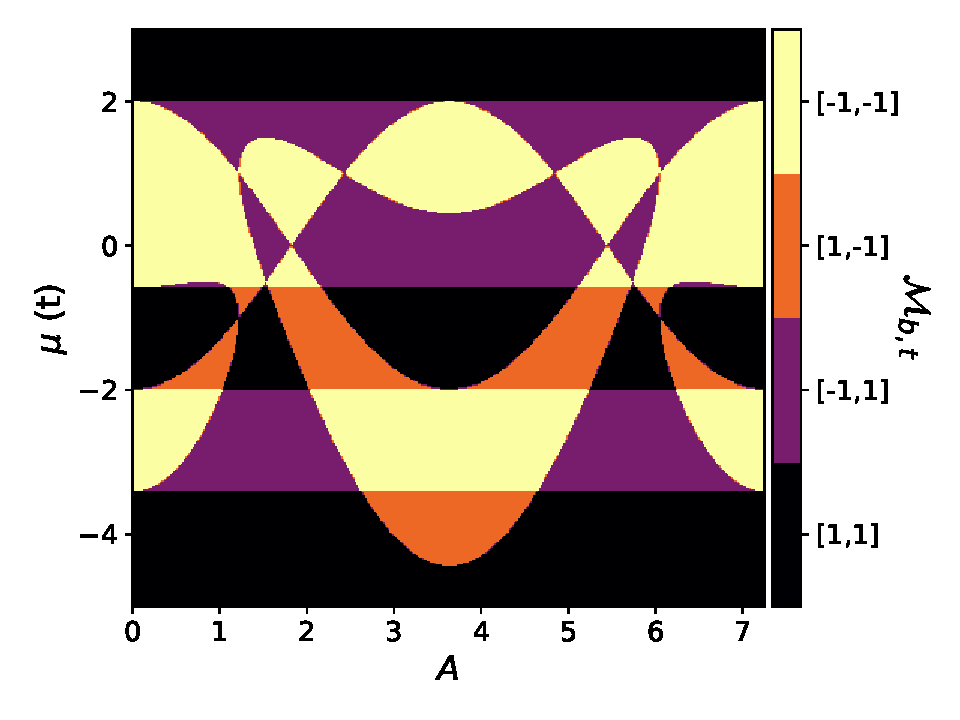
\includegraphics[width=0.55\textwidth]{./figures/supp/topological-phase-diagram-1pi3-w-3.pdf}} \\
  \vspace{-20pt}
  \subfloat[]{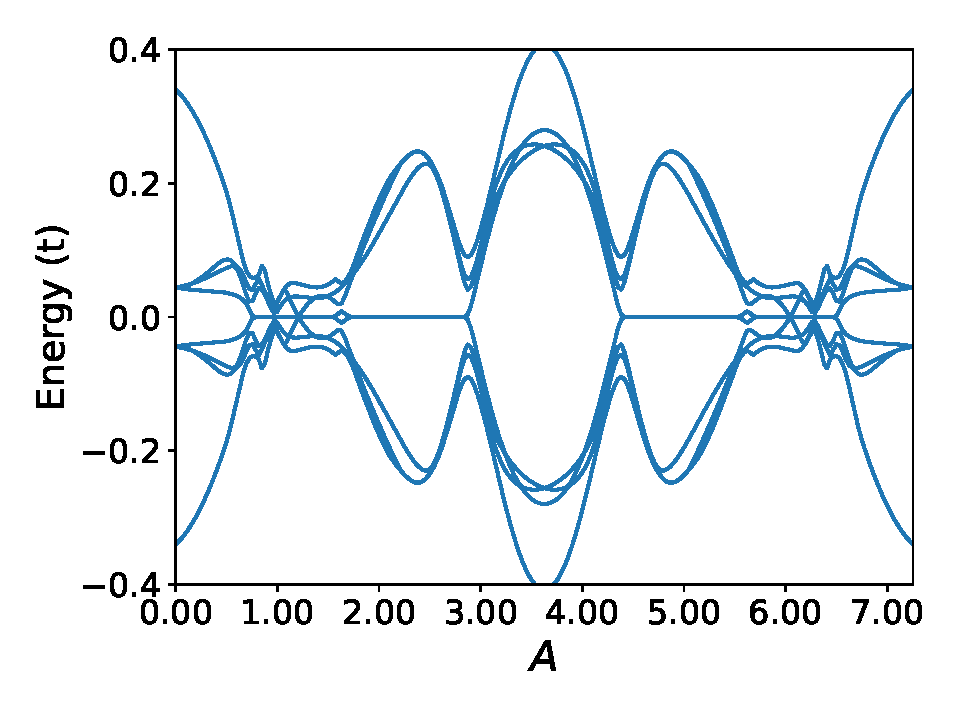
\includegraphics[width=0.46\textwidth]{./figures/supp/spectral-flow-nr-80-w-3-mu-1_6000.pdf}} \\
  \hspace{70pt}
  \subfloat[]{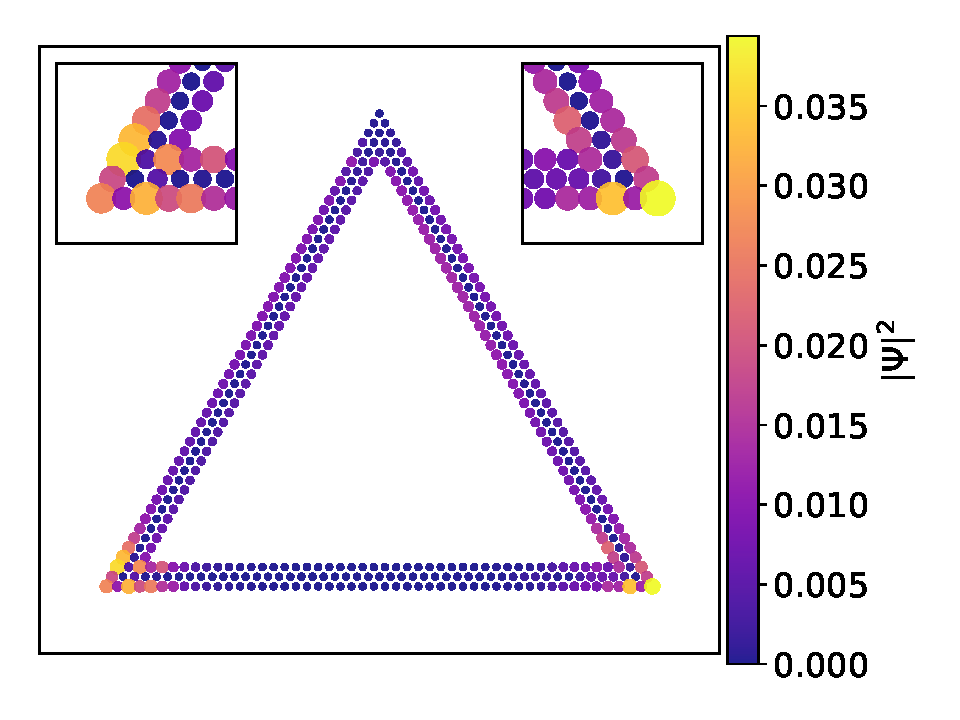
\includegraphics[width=0.45\textwidth]{./figures/supp/GS-A-2_74-nr-50-w-3-mu-1_6.pdf}}
  \caption{(a) Topological phase diagram for a $W=3$ hollow triangle obtained by overlapping the $\mathcal{M}_{t,b}(A, \mu)$ plots of 1D chains with $\mathbf A = A\hat{y}$ and $\mathbf A = A(\frac{\sqrt{3}}{2}\hat{x}+\frac{1}{2}\hat{y})$. Color scheme: purple---$[\mathcal{M}_t,\mathcal{M}_b]=[1,1]$, yellow---$[\mathcal{M}_t,\mathcal{M}_b]=[-1,-1]$, red---$[\mathcal{M}_t,\mathcal{M}_b]=[1,-1]$, orange---$[\mathcal{M}_t,\mathcal{M}_b] = [-1,1]$ (b) Near-gap BdG eigen-energies vs $A$ for a finite triangle with edge length $L=50$, $W=3$, and $\mu=1.6$. (c) BdG eigenfunction $|\Psi|^2$ summed over the two zero modes at $A=2.4709$.}
  \label{fig: supp pd}
\end{figure}

A model that is closer to a realistic hollow triangular island is the finite-width triangular chain or ribbon. An example, illustrated in Figure \ref{fig: supp pd} (c), has its edge length $L=50$ and width $W=3$. The phase diagram Fig.~\ref{fig: supp pd} (a) is created in a similar way as that in Fig.~3 (b) of the main text, assuming a constant vector potential along $\hat{y}$ and infinitely long $W=3$ ribbons. The spectral flow for the actual triangle with $\mu = 1.6$ in Fig.~\ref{fig: supp pd} (b) shows MZM in the parameter regions in agreement with the phase diagram. Fig.~\ref{fig: supp pd} (c) plots the MZM wavefunction for $A=2.4709$ and $\mu=1.6$ that are indeed well localized at the bottom corners.

\begin{figure}[ht]
  \hspace{-20pt}
  \subfloat[]{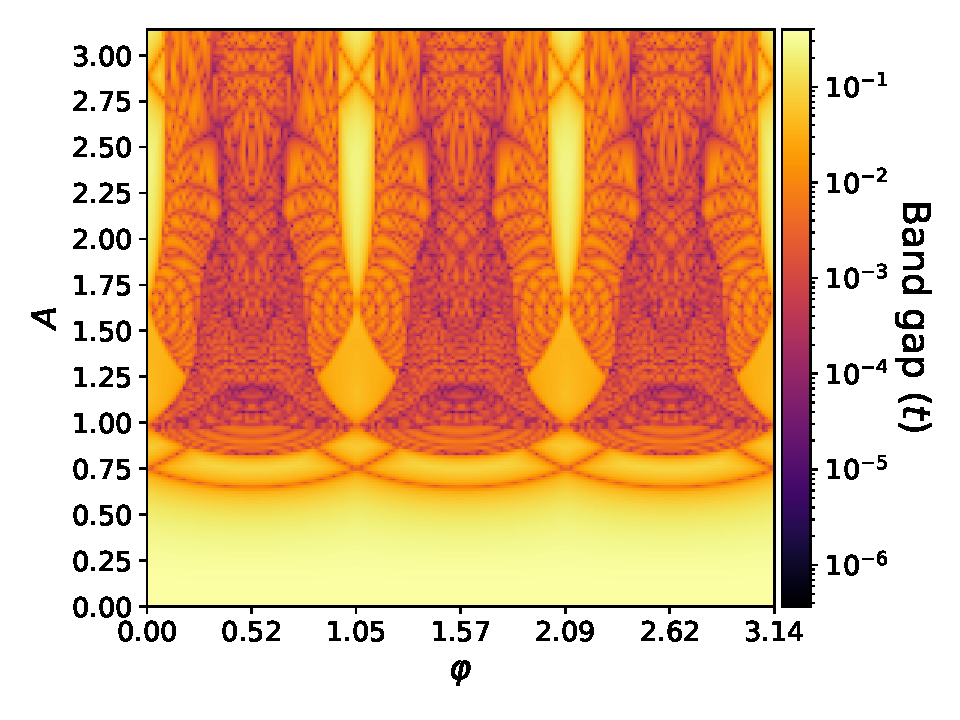
\includegraphics[width=0.4\textwidth]{./figures/supp/band-gap-rotation-w-3-mu-p1_6000.pdf}}
  \subfloat[]{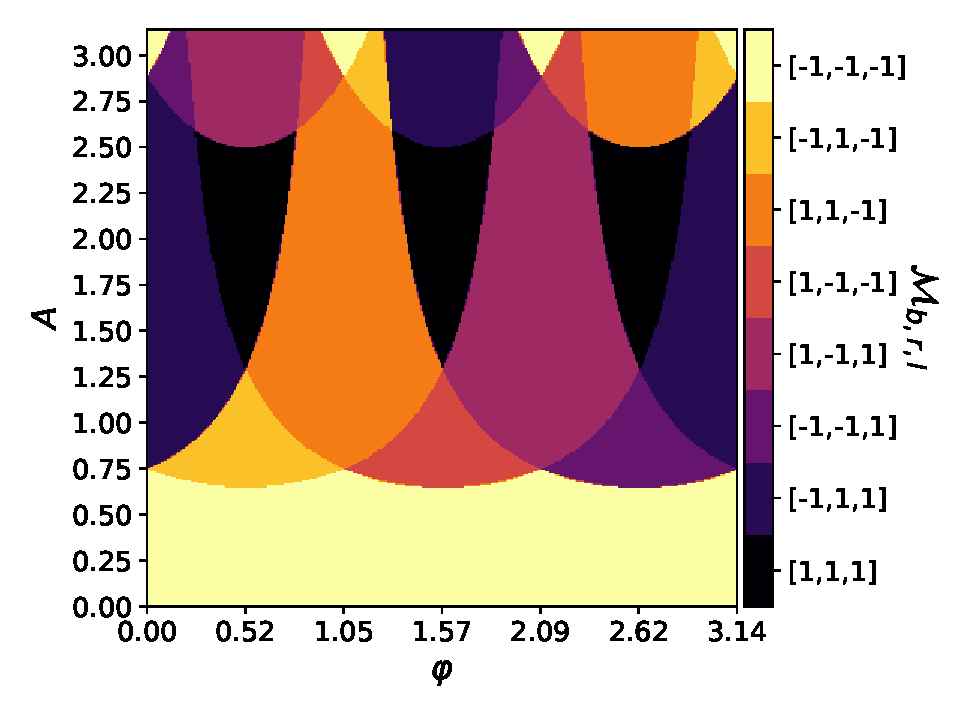
\includegraphics[width=0.4\textwidth]{./figures/supp/topological-phase-diagram-w-3-mu-p1_6000.pdf}}\\
  \subfloat[]{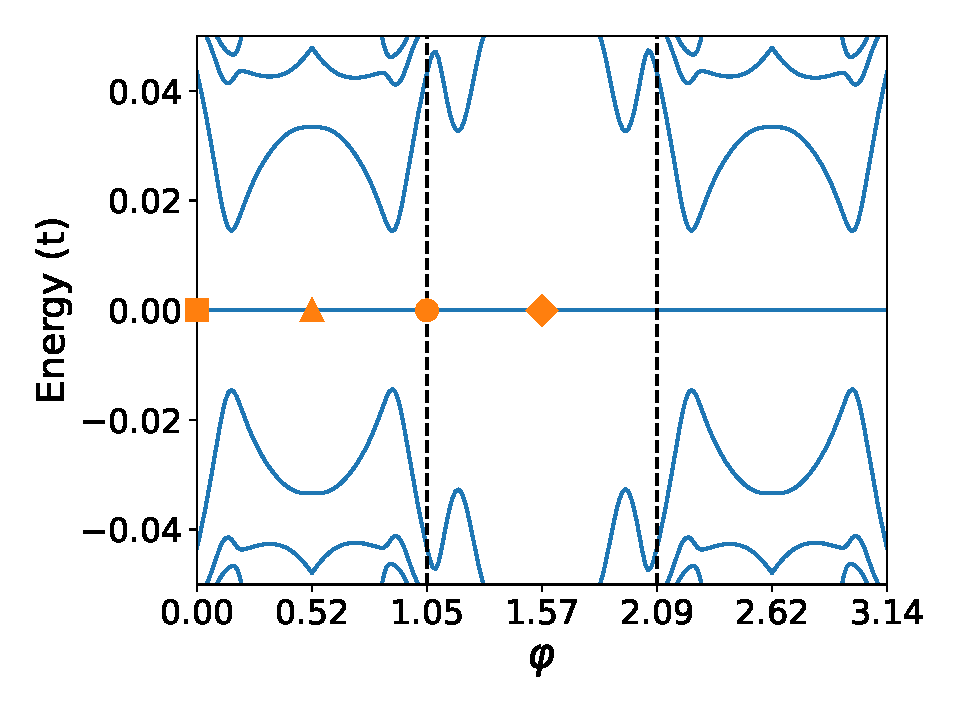
\includegraphics[width=0.4\textwidth]{./figures/supp/spectral-flow-nr-80-w-3-mu-p1_6000.pdf}}\\
  \subfloat[]{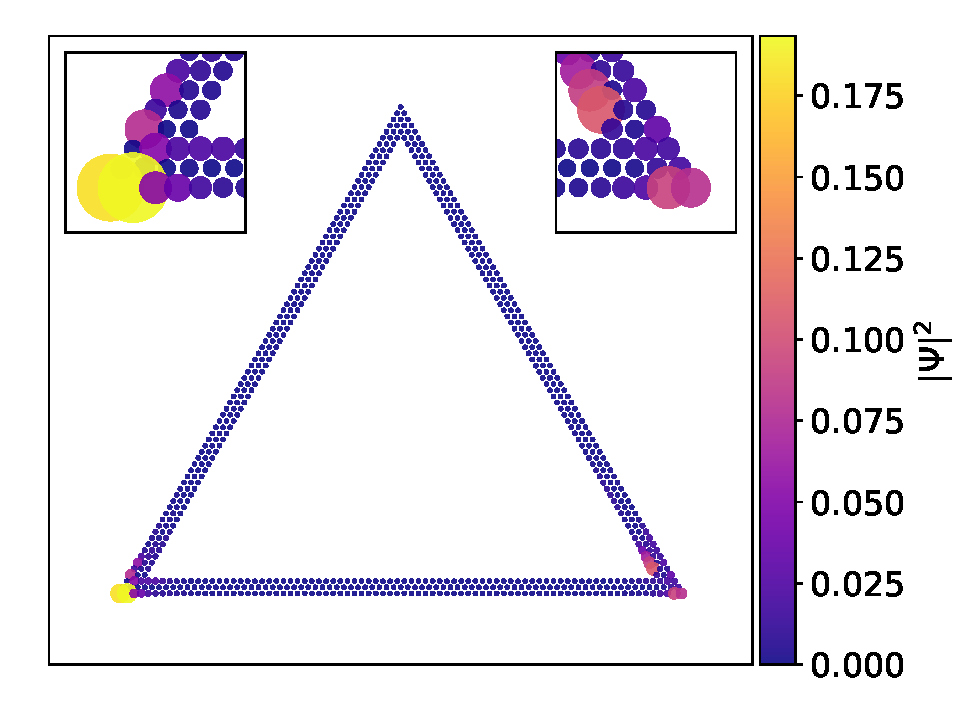
\includegraphics[width=0.35\textwidth]{./figures/supp/GS-T-Square-w-3.pdf}}
  \subfloat[]{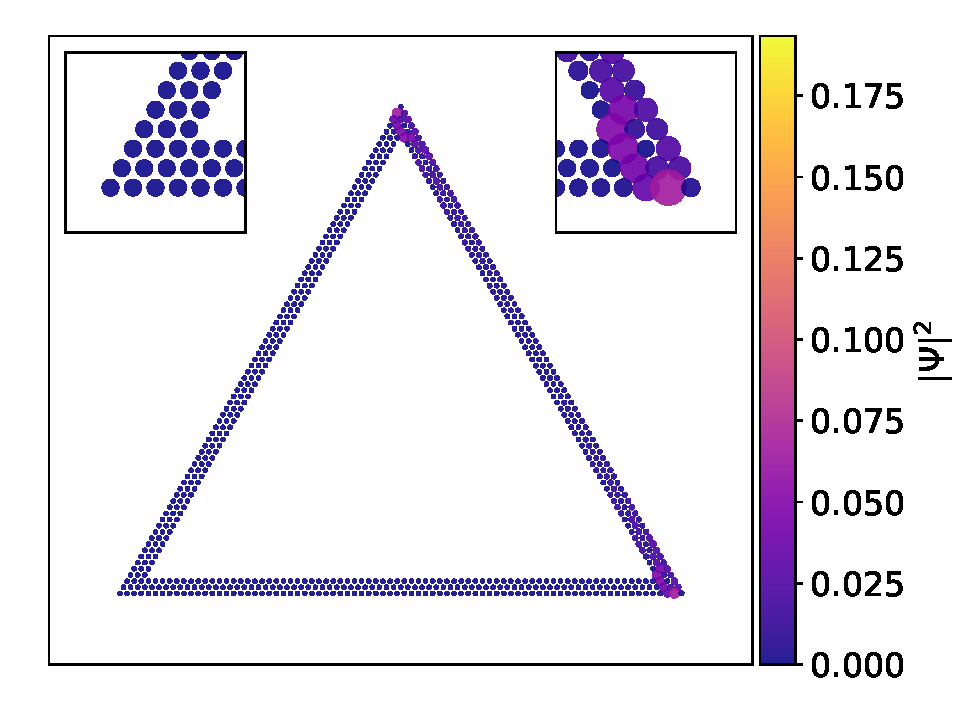
\includegraphics[width=0.35\textwidth]{./figures/supp/GS-T-Triangle-w-3.pdf}}\\
  \subfloat[]{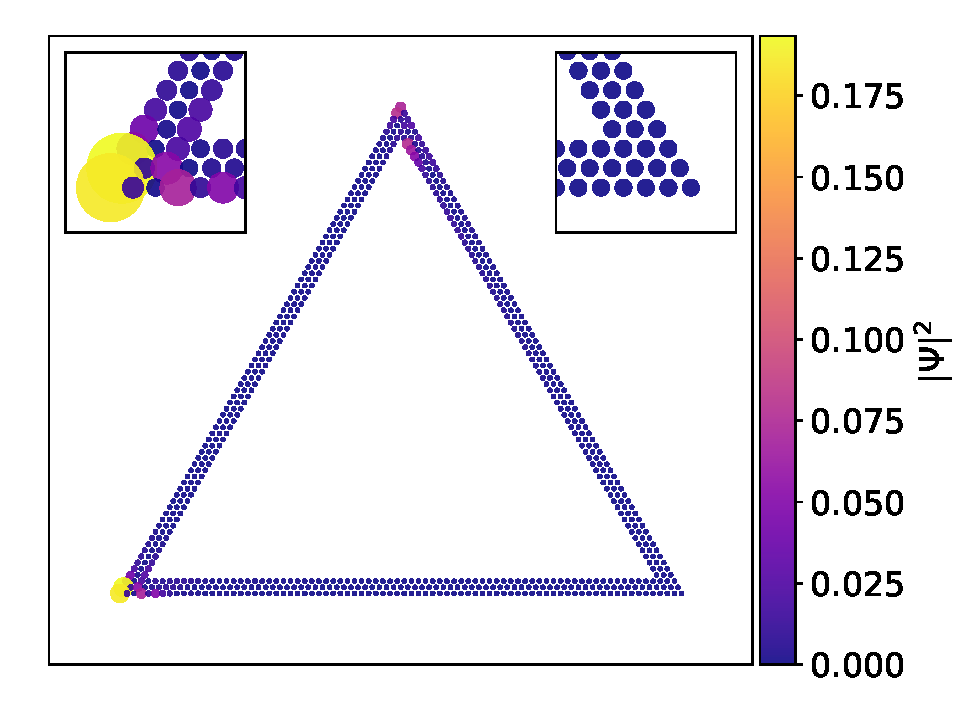
\includegraphics[width=0.35\textwidth]{./figures/supp/GS-T-Circle-w-3.pdf}}
  \subfloat[]{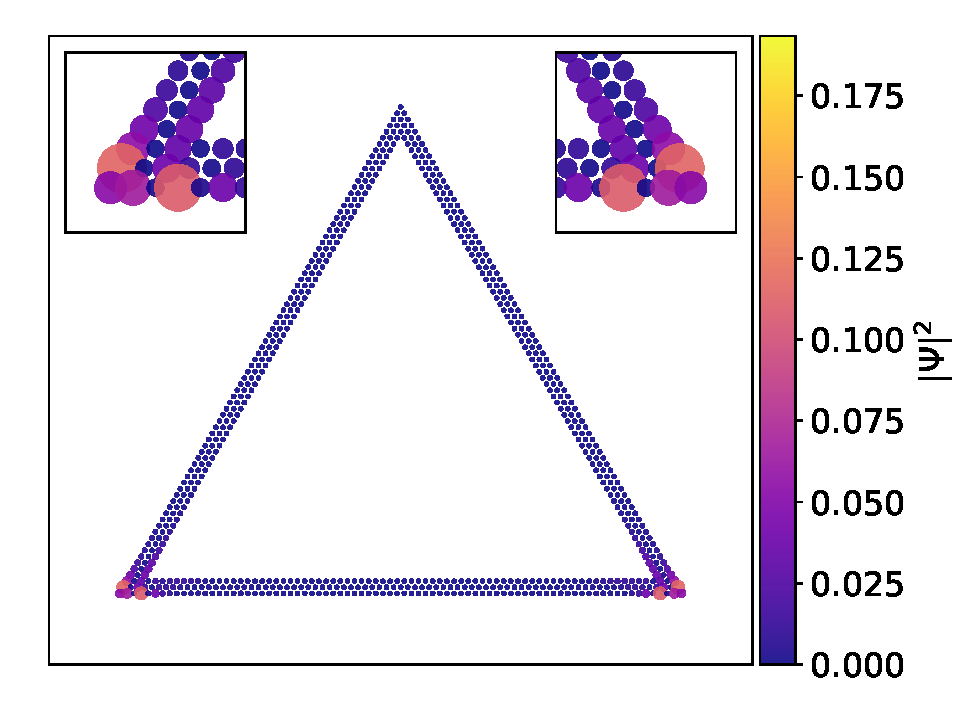
\includegraphics[width=0.35
\textwidth]{./figures/supp/GS-T-Diamond-w-3.pdf}}
  \caption{(a) Spectral flow of a hollow triangle with $W=3$, $L=50$, $\mu=1.6$, and $A=2.75$ with increasing rotation angle $\varphi$, defined through $\mathbf A = A(-\sin\varphi \hat{x} + \cos\varphi \hat{y})$. (b-c) BdG eigenfunction $|\Psi|^2$ summed over the two zero modes at $\varphi = 0$ and $\frac{\pi}{3}$, respectively.}
  \label{fig: supp rotation}
\end{figure}

We next discuss how to move the MZM on a hollow triangle by rotating the vector potential. Due to the Peierls phase accumulated by hopping that is not parallel with the ribbon edges for general width ribbons, the vector potential has a more complex effect on the energy spectrum than that for the $W=1$ case. To ensure that the bulk band gap of individual edges only closes at a few isolated topological phase transition points, we plot in Figure~\ref{fig: supp rotation} (a) the smallest gap of the three edges with periodic boundary condition versus $(A,\varphi)$. One can see that 

shows the spectral flow and eigenfunctions as we rotate $\varphi=0$ to $\varphi=\pi$ counterclockwisely. The two MZM cycle through the three vertices in a similar manner as that in Fig.~4 of the main text (only the MZM wavefunctions at $\varphi = 0$ and $\frac{\pi}{3}$ are plotted as representatives of the $\varphi = n\pi/3$ cases). Note that the spectral flow has 3-fold rotation symmetry but not 6-fold, since increasing $\varphi$ by $\frac{2\pi}{3}$ is equivalent to rotating the coordinate system clockwisely by $\frac{2\pi}{3}$. In contrast, rotating the vector potential by $\frac{\pi}{3}$, if without an additional sign change of the $p$-wave pairing potential, is not an exact symmetry of the finite triangle. Also we did not try to scrutinize the phase diagram to find a parameter path in which the bulk gap does not close, as in the $W=1$ case in the main text. Here we just point out that identifying a system-specific parameter path for adiabatic manipulation of MZM is in principle always possible, especially if one is allowed to have more knobs other than $\varphi$ in real structures, such as tuning the chemical potential of individual edges or the size of the vector potential, etc.

\section{Braiding MZM in a small network of triangles}

In this section we show that one can braid two out of four MZM, a minimal setting for nontrivial manipulation of the degenerate many-body ground states, by using a small network of corner-sharing triangles. We focus on the critical step of swapping $\gamma_2$ and $\gamma_3$ as labeled in Fig.~5 of the main text. This can be done by rotating the vector potential of the triangle in the middle of the bottom row from $\varphi = \frac{\pi}{6}$ to $\frac{\pi}{3}$. More specifically, when $\varphi = \frac{\pi}{6}$, with the chosen values of $\mu$ and $A$, only the right edge of the said triangle is topologically nontrivial. The chain that hosts $\gamma_{3,4}$ thus extends through this nontrivial edge to the top triangle as in Fig.~\ref{fig: supp braiding} (b). On the other hand, when $\varphi$ increases to $\frac{\pi}{3}$, the nontrivial edge of the middle triangle changes from right to left, which leads to $\gamma_2$ hopping from its left corner to the right through the top corner, while $\gamma_3$ is unaffected [Figs.~\ref{fig: supp braiding} (c-g)]. As a result the $\gamma_2,\gamma_3$ swapping is done without closing the bulk gap, as can be seen from the spectral flow in Fig.~\ref{fig: supp braiding} (a).

\begin{figure}
  \hspace{-30pt}
  \subfloat[]{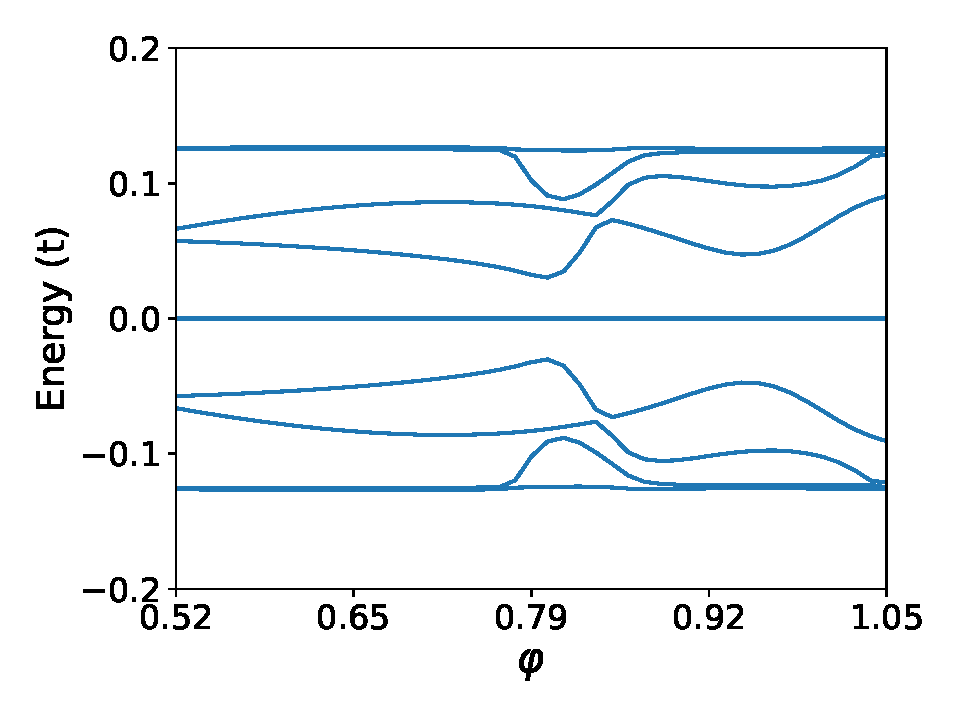
\includegraphics[width=0.5\textwidth]{./figures/supp/spectral-flow-braiding.pdf}} \\
  \subfloat[]{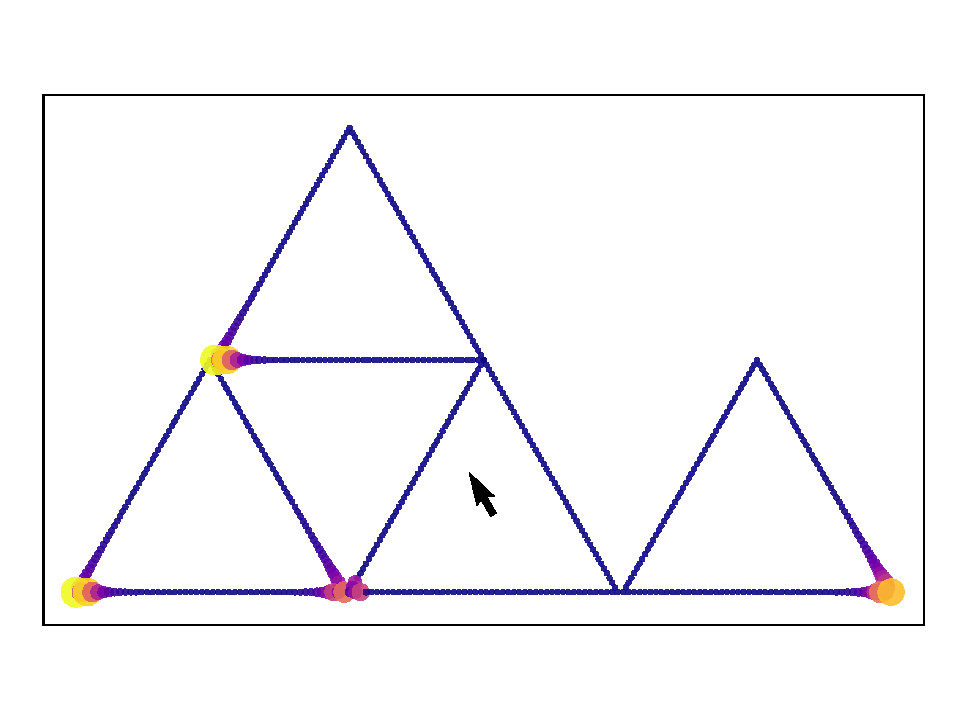
\includegraphics[width=0.35\textwidth]{./figures/supp/GS-T-0_5236.pdf}}
  \subfloat[]{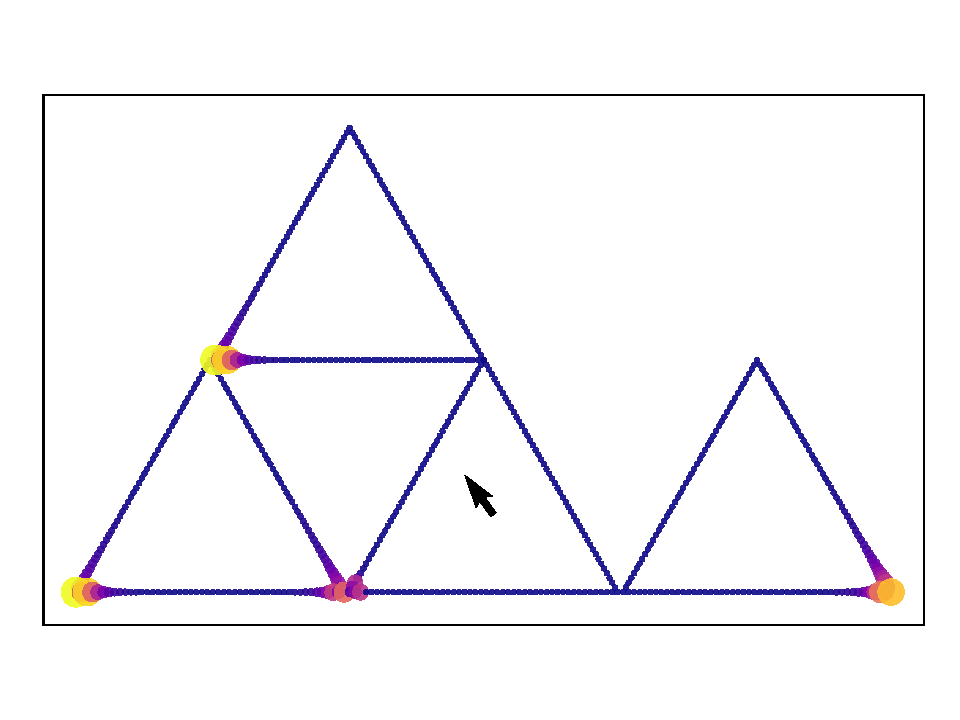
\includegraphics[width=0.35\textwidth]{./figures/supp/GS-T-0_6283.pdf}} \\
  \subfloat[]{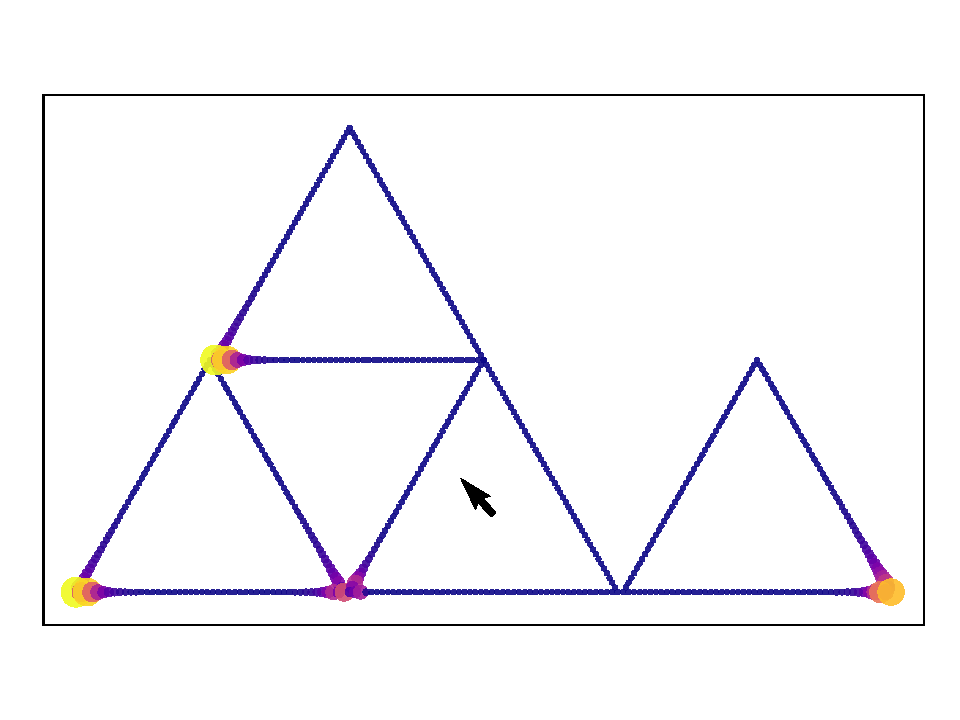
\includegraphics[width=0.35\textwidth]{./figures/supp/GS-T-0_7330.pdf}}
  \subfloat[]{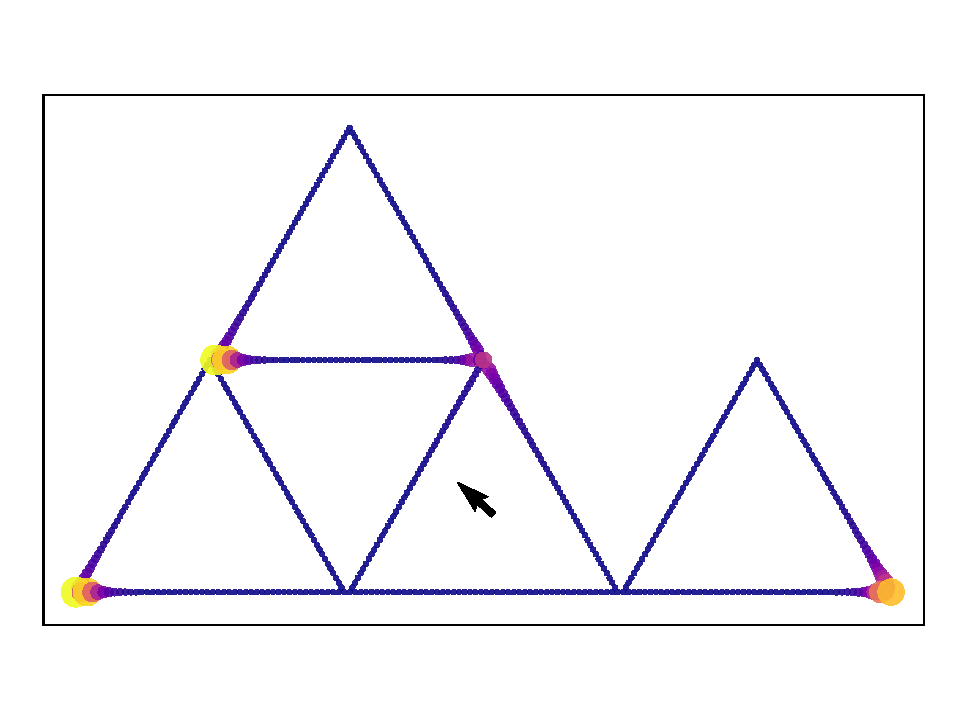
\includegraphics[width=0.35\textwidth]{./figures/supp/GS-T-0_8378.pdf}} \\
  \subfloat[]{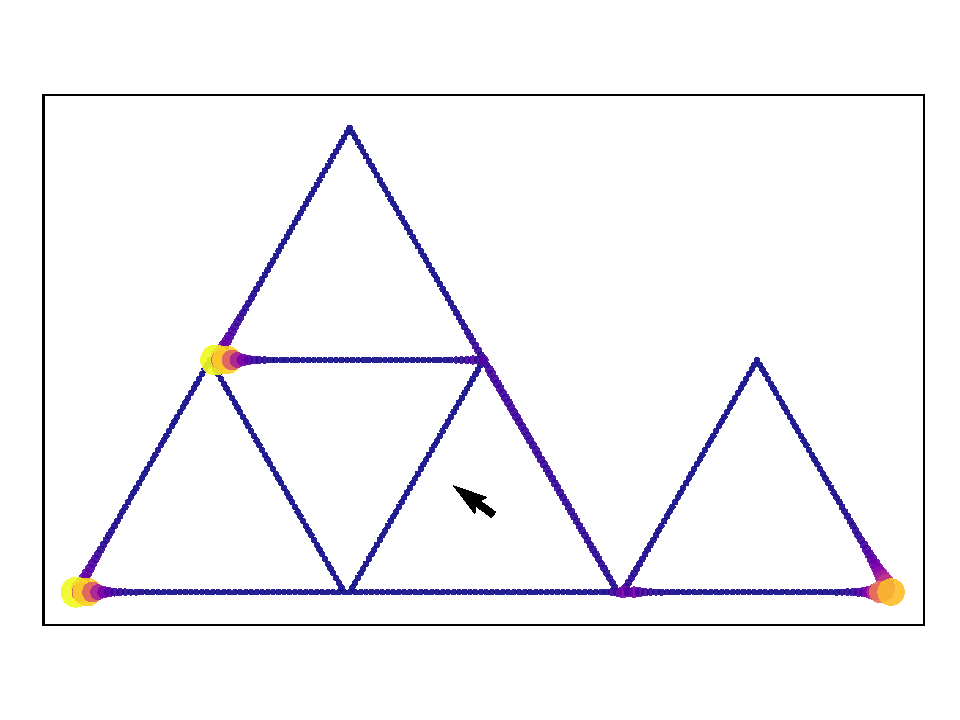
\includegraphics[width=0.35\textwidth]{./figures/supp/GS-T-0_9425.pdf}}
  \subfloat[]{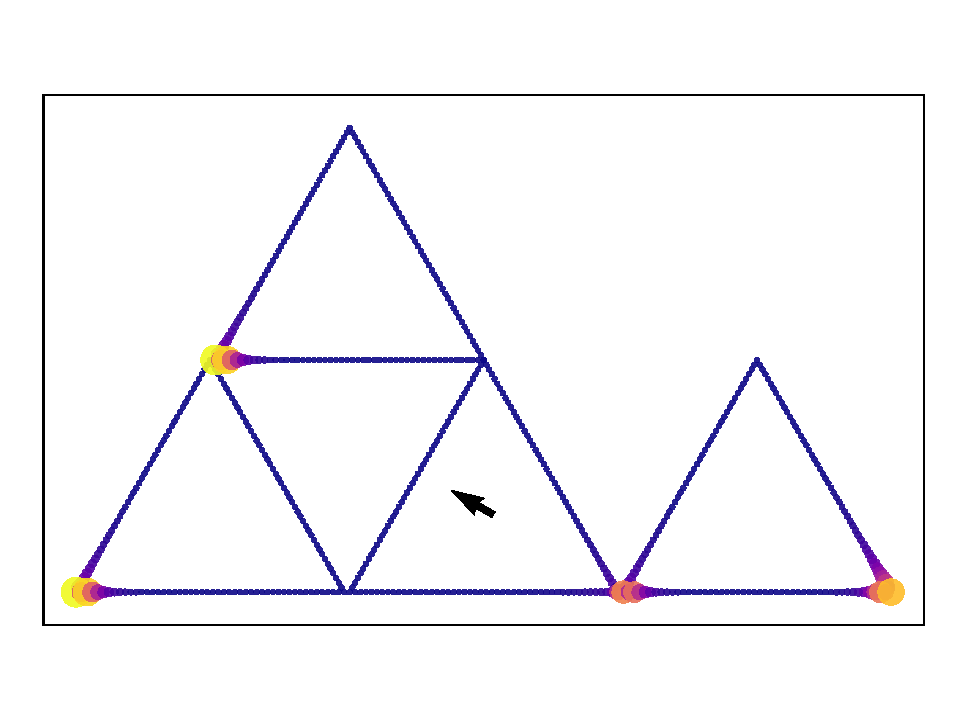
\includegraphics[width=0.35\textwidth]{./figures/supp/GS-T-1_0472.pdf}}
  \caption{(a) Spectral flow for the critical step of swapping $\gamma_2$ and $\gamma_3$ in the example of Fig.~5 in the main text, calculated using four corner-sharing triangles of $W=1$ and $L=50$, with $\mu=1.6$ and $A=2.6$. Vector potential for the middle triangle in the bottom row can rotate according to $\mathbf A = A(-\sin\varphi \hat{x} + \cos\varphi \hat{y})$ from $\varphi = \frac{\pi}{6}$ to $\frac{\pi}{3}$, while the other three have fixed $\varphi = 0$. (b)-(g) BdG eigenfunction $|\Psi|^2$ summed over the four zero modes at equally-spaced points along the rotation path. The black arrow indicates the direction of the vector potential for the bottom middle triangle.}\label{fig: supp braiding}
\end{figure}

\bibliography{triag_cite}

\end{document}
